
\chapter{基于主动感知的多智能体交通资产检测框架}
\label{chap:active_perception_framework}

\section{引言}
\label{sec:active_perception_intro}

交通资产检测是道路数字化管理、资产清查与智能运维中的关键基础任务，其目标在于从复杂道路场景中自动识别并定位路灯、交通标志、交通锥桶、井盖、消火栓以及监控设施等多类交通资产。与通用目标检测场景相比，交通资产检测具有更为显著的多尺度、稠密分布与局部易漏检特征：一方面，不同类别资产在几何尺寸、外观形态与空间分布上存在较大差异；另一方面，远距离小目标、密集分布目标以及位于图像边缘区域的目标，往往更容易受到背景干扰、尺度压缩与局部遮挡等因素影响，从而导致检测器出现漏检、重复检测或定位偏差等问题。

现有目标检测方法大多采用单阶段或双阶段的统一检测范式，即在单次全图前向推理中完成特征提取、候选生成与边界框回归。这类方法在显著目标检测上通常能够获得较好效果，但对于交通资产场景中普遍存在的小目标、密集目标与疑难区域，其检测性能往往受限于全局输入尺度和统一感受野建模方式。换言之，单次全图检测更倾向于优先关注显著区域，而缺乏对潜在遗漏区域进行再次观察与主动补充的机制。

针对上述问题，本文提出一种\textbf{基于主动感知的多智能体交通资产检测框架}。该框架将交通资产检测过程由传统的单次静态推理重构为“\textbf{全局初检—候选区域推荐—局部精检—结果融合}”的三阶段主动感知流程。在该框架中，系统由两类功能异质但协同工作的智能体共同构成：其一为检测 Agent（Detection Agent），负责在全图或局部裁剪区域中执行目标检测；其二为裁剪 Agent（Crop Agent），负责根据场景内容与初步检测结果主动生成具有高补检价值的候选区域。二者通过阶段化协作形成闭环，使检测系统具备对潜在遗漏区域进行主动再感知的能力。

本文研究按照“先同源训练、再异构替换”的两阶段路线展开，具体如下。第一阶段（同源训练阶段）：Detection Agent 与 Crop Agent 均基于 rexomini 训练得到，并采用强化学习方式分别优化“检测框匹配质量”和“候选裁剪区域价值”，以完成三阶段主动感知流程能力构建。第二阶段（异构替换阶段）：在第一阶段已验证三阶段流程有效的前提下，仅替换第一、三阶段的 Detection Agent，Crop Agent 保持固定，用于评估框架的检测器无关性。rexomini 是一个 3B 参数规模的多模态检测模型，构建于 Qwen2.5-VL-3B-Instruct 之上，通过将坐标离散化为专用 token 实现文本化坐标预测，并采用“SFT 预训练 + GRPO 强化后训练”的两阶段训练范式以提升定位精度与输出行为稳定性\cite{rexomni2025}。

本文在同源训练阶段选用 rexomini 作为核心 Detection Agent，并以其继续训练得到 Crop Agent，主要基于以下考虑：其一，rexomini 属于生成式多模态检测模型，能够以坐标 token 形式输出检测结果，与本文“全局初检—候选区域推荐—局部精检—结果融合”的主动感知流程具有较好的接口一致性；其二，该模型构建于 Qwen2.5-VL-3B-Instruct 之上，具备较强的视觉—语言联合建模能力，有利于与后续属性识别阶段形成统一的多模态技术路线；其三，rexomini 采用“SFT 预训练 + GRPO 强化后训练”的训练范式，能够为本文所设计的 \texttt{BoxIoURewardFunction} 与 \texttt{CropRegionRewardFunction} 提供较稳定的优化基础；其四，Crop Agent 的任务本质上是候选区域决策，由已具备目标位置感知能力的 Detection Agent 继续训练得到，有助于提升候选区域推荐的训练稳定性与收敛性。基于上述原因，本文采用 rexomini 完成同源训练阶段的方法构建，并在固定 Crop Agent 的前提下进一步开展异构 Detection Agent 的替换实验。

进一步地，本文框架中的 Detection Agent 并不依赖于单一模型实现，而可以根据实际需求替换为大模型检测器或现有目标检测模型，例如 DINO\cite{zhang2022dino}、Faster R-CNN\cite{ren2015faster}、DEIM\cite{huang2025deim}、Grounding DINO\cite{liu2024grounding} 和 YOLO26\cite{ultralytics2026yolo26}。因此，该方法并非某一特定模型的附属优化技巧，而是一种具有较强模型无关性与可迁移性的检测增强框架。第四章将在统一流程下对这种可替换性进行定量验证。

% ========================= 图 4-1 =========================
\begin{figure}[htbp]
    \centering
    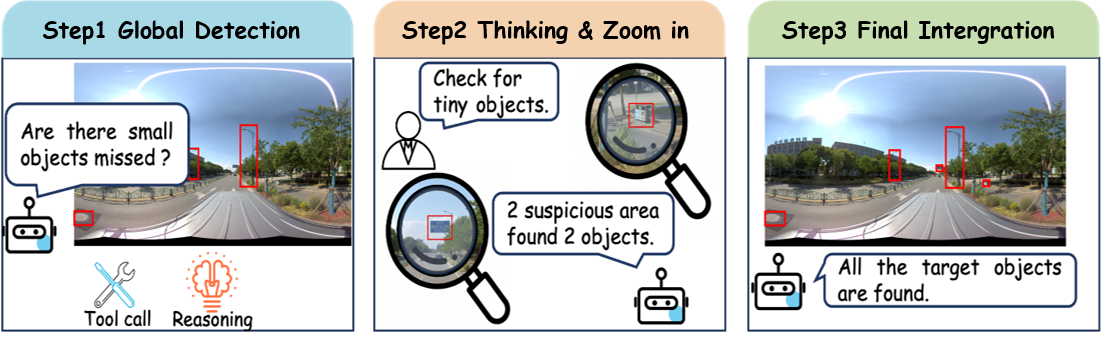
\includegraphics[width=\textwidth]{logo/三阶段检测框架图.png}
    \caption{基于主动感知的多智能体交通资产检测框架总体示意图}
    \label{fig:framework_overview}
\end{figure}
% =========================================================


\section{基于异构 Agent 协作的三阶段检测框架}
\label{sec:heterogeneous_agents_framework}

\subsection{问题定义与框架概述}
\label{subsec:problem_definition_framework_overview}

设输入道路场景图像为 $I$，目标是输出图像中全部交通资产的类别标签与边界框集合。与传统检测器直接建立从 $I$ 到检测结果的单步映射不同，本文将检测过程拆分为三个阶段，并引入裁剪 Agent 与检测 Agent 的协同机制。

第一阶段中，Detection Agent 在整幅图像上执行全局检测，得到初始检测结果集合：
\begin{equation}
\mathcal{B}^{(1)} = f_{\text{det}}^{(1)}(I),
\label{eq:stage1_detection}
\end{equation}
其中，$\mathcal{B}^{(1)}$ 表示第一阶段输出的边界框集合，$f_{\text{det}}^{(1)}(\cdot)$ 表示第一阶段检测模型。

第二阶段中，Crop Agent 根据原始图像与第一阶段检测结果，生成候选裁剪区域集合：
\begin{equation}
\mathcal{C} = f_{\text{crop}}(I, \mathcal{B}^{(1)}),
\label{eq:stage2_crop}
\end{equation}
其中，$\mathcal{C}=\{c_1,c_2,\dots,c_N\}$ 表示候选裁剪区域集合，$f_{\text{crop}}(\cdot)$ 表示裁剪 Agent。

第三阶段中，Detection Agent 在每个裁剪区域上执行局部检测，得到局部补检结果：
\begin{equation}
\mathcal{B}^{(3)} = \bigcup_{c_i \in \mathcal{C}} f_{\text{det}}^{(3)}(I_{c_i}),
\label{eq:stage3_detection}
\end{equation}
其中，$I_{c_i}$ 表示由候选区域 $c_i$ 从原图中裁剪得到的局部图像，$\mathcal{B}^{(3)}$ 表示第三阶段检测结果集合。

最终，系统对第一阶段与第三阶段结果进行融合，得到最终输出：
\begin{equation}
\mathcal{B}^{*} = \mathcal{F}\left(\mathcal{B}^{(1)}, \mathcal{B}^{(3)}\right),
\label{eq:final_fusion_general}
\end{equation}
其中，$\mathcal{F}(\cdot)$ 表示后处理融合函数。

从整体上看，本文方法并不是简单地在原有检测流程后附加一个额外检测步骤，而是通过裁剪 Agent 主动识别潜在高价值区域，再由检测 Agent 在局部尺度下进行补充检测，从而将目标检测过程由“单次静态识别”扩展为“面向遗漏区域的主动搜索”。

\subsection{Detection Agent 与 Crop Agent 的功能分工}
\label{subsec:agent_roles}

在本文框架中，Detection Agent 与 Crop Agent 在功能上并不重叠，而是形成了清晰的任务分工。

Detection Agent 的主要职责是“\textbf{识别并定位目标}”。在第一阶段中，它负责完成场景级全局初检，获取显著目标与易检目标的初始结果；在第三阶段中，它负责在局部裁剪区域内执行补充检测，以恢复第一阶段中可能漏检的目标。因此，Detection Agent 同时承担了全局感知与局部精检两种功能，但其作用方式在两个阶段中并不相同：第一阶段强调全局覆盖，第三阶段强调局部补检。

Crop Agent 的主要职责是“\textbf{决定哪里值得再看}”。它并不直接输出最终目标框，而是根据原图内容与第一阶段检测结果，生成若干具有高补检价值的局部候选区域。这些区域往往对应于小目标聚集区域、密集目标区域、边缘疑难区域或潜在漏检区域。也就是说，Crop Agent 实际上承担的是一种主动感知中的“注意力重分配”角色，其输出将直接决定第三阶段检测的重点范围。

因此，本文框架中两个 Agent 的协同逻辑可以概括为：Detection Agent 负责“\textbf{看见目标}”，Crop Agent 负责“\textbf{发现值得再次观察的区域}”。通过这种分工，系统不再依赖单一模型在单次前向中同时完成全局扫描与局部精检，而是将二者解耦为具有明确职责边界的两个功能模块。

\subsection{Detection Agent 的异构可替换性}
\label{subsec:heterogeneous_detection_agent}

本文框架的重要特点之一在于 Detection Agent 的可替换性。由于 Crop Agent 的任务是输出候选区域，而 Detection Agent 的任务是在给定图像或局部区域中输出检测框，因此二者并不需要共享相同的模型架构。只要某一检测模型能够接受图像输入并输出目标类别与边界框，它便可作为 Detection Agent 接入本文所提出的三阶段主动感知流程。

基于这一特点，第一阶段和第三阶段的 Detection Agent 既可以采用基于视觉语言大模型的检测模型，也可以替换为现有目标检测器，例如 YOLO、DINO、Grounding DINO 等。训练策略上，本文采用分情形设定：当 Detection Agent 为 rexomini 时，使用 \texttt{BoxIoURewardFunction} 进行强化学习训练以增强模型对小物体的感知力；当 Detection Agent 替换为其他检测模型时，均沿用各自模型原始训练方式，不额外施加本文强化学习奖励。需要强调的是，第二阶段 Crop Agent 在本文中不进行异构替换：一方面其输出是“候选裁剪区域策略”，而非普通检测框；另一方面现有对比检测器通常只具备目标检测能力，不具备可直接替代的 Crop 决策能力。此时，本文方法不再依赖于具体检测器内部结构，而是在更高层次上为不同检测器提供统一的主动感知补检机制。因此，本文框架实质上是一种面向多种检测器的检测增强范式，而非仅适用于某一特定模型的专用策略。

这一异构可替换性带来的直接意义在于：一方面，系统能够根据实际需求在检测精度、开放词汇能力与模型复杂度之间进行灵活配置；另一方面，也使本文方法具备更强的工程可扩展性与实验泛化性，为后续验证其在多种检测模型上的一致有效性提供了基础。需要说明的是，本文在实验阶段为保证变量可控，固定第二阶段 Crop Agent，仅替换第一、三阶段 Detection Agent。

% ========================= 图 4-2 =========================
\begin{figure}[htbp]
    \centering
    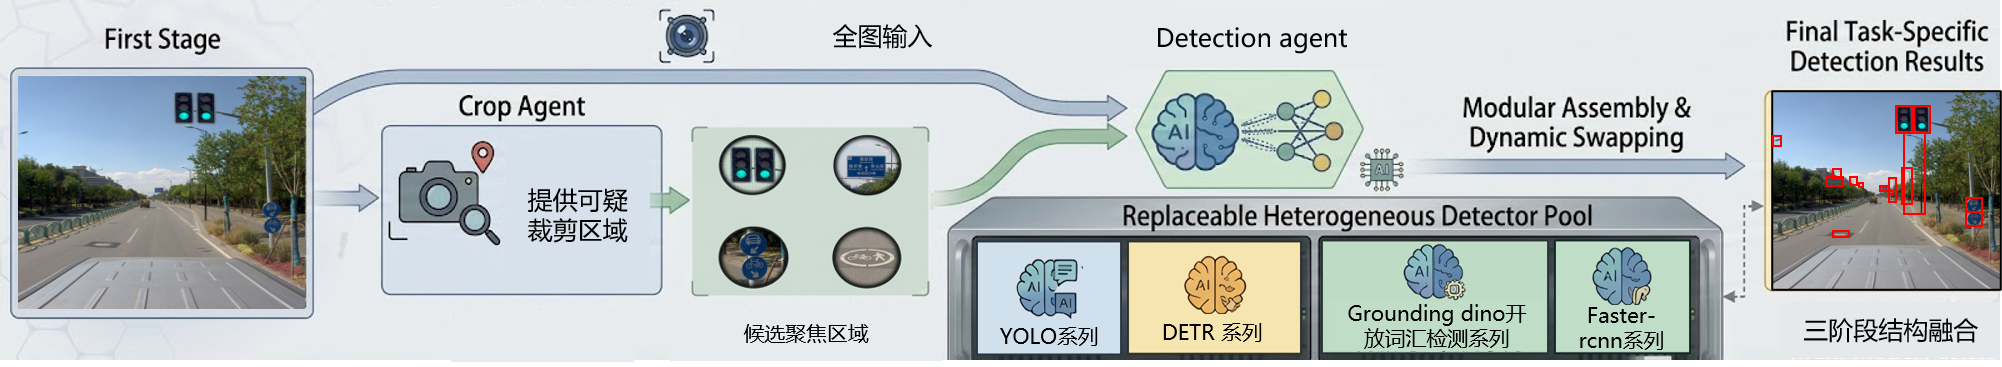
\includegraphics[width=1.0\textwidth]{logo/裁剪 Agent 与异构 Detection Agent 的协作关系示意图.png}
    \caption{裁剪 Agent 与异构 Detection Agent 的协作关系示意图}
    \label{fig:heterogeneous_agents}
\end{figure}
% =========================================================


\section{第一阶段：面向全局场景的初步检测}
\label{sec:stage1_global_detection}

\subsection{全局检测阶段的作用}
\label{subsec:role_of_global_detection}

第一阶段的目标是在整幅图像上执行初步检测，以建立场景中交通资产分布的初始估计。该阶段承担的是场景级粗粒度感知任务，其主要作用包括以下三个方面。

首先，第一阶段为最终检测结果提供基础框集合。全图检测能够优先识别场景中显著性较强、尺度较大或局部特征较为清晰的目标，从而形成一组覆盖主要交通资产的初始结果。

其次，第一阶段为后续主动裁剪提供参考。Crop Agent 在第二阶段生成候选区域时，并不是脱离检测结果进行独立裁剪，而是综合利用原始图像内容与第一阶段检测结果来判断潜在遗漏区域。因此，第一阶段输出的质量将直接影响第二阶段区域推荐的有效性。

最后，第一阶段为后续局部补检定义了“待补充空间”。本文方法的目标并不是通过第一阶段一次性穷尽全部目标，而是先建立一个较为可靠的全局基线，再借助后续主动裁剪与局部精检对疑难区域进行补充。因此，第一阶段的价值更多体现在全局覆盖与先验提供，而非单独完成全部检测任务。

\subsection{Detection Agent 的训练目标}
\label{subsec:detection_agent_training_objective}

为了提升 Detection Agent 在全图与局部区域中的检测能力，本文在 “Detection Agent=rexomini” 的设置下，先构造基于框匹配质量的检测奖励机制，再将其实现为 \texttt{BoxIoURewardFunction} 用于强化学习训练。该奖励函数并不简单依赖传统的离散 TP/FP 统计，而是通过连续几何匹配信号与小目标增强机制，为模型训练提供更加细粒度的优化引导。对于后续替换的 DINO、Faster R-CNN、DEIM、Grounding DINO 和 YOLO26，本文均使用其原始训练范式，不使用本节奖励函数进行再训练，故不再赘述。

设真实框为 $b^g$，预测框为 $b^p$，则二者的交并比（Intersection over Union, IoU）定义为：
\begin{equation}
\mathrm{IoU}(b^g, b^p)=\frac{|b^g\cap b^p|}{|b^g\cup b^p|}.
\label{eq:iou}
\end{equation}

为了在预测框与真实框不相交时仍能提供有效优化信号，本文在匹配阶段引入广义交并比（Generalized IoU, GIoU）：
\begin{equation}
\mathrm{GIoU}(b^g,b^p)
=
\mathrm{IoU}(b^g,b^p)
-
\frac{|C|-|b^g\cup b^p|}{|C|},
\label{eq:giou}
\end{equation}
其中，$C$ 表示同时包围 $b^g$ 与 $b^p$ 的最小外接框区域。基于 GIoU 构造匹配代价矩阵后，采用匈牙利算法建立预测框与真实框之间的一一匹配关系，以避免多个预测框重复对应同一真实目标。

在完成匹配后，本文使用 IoU 作为基本匹配得分。同时考虑到交通资产场景中小目标更易漏检、定位更敏感，本文对小目标引入更高权重。设真实框面积为 $A_i$，当其小于小目标阈值 $A_{\text{small}}$ 时，赋予其更高权重：
\begin{equation}
w_i=
\begin{cases}
\lambda_s, & A_i < A_{\text{small}},\\
1, & \text{otherwise},
\end{cases}
\label{eq:small_object_weight}
\end{equation}
其中，$\lambda_s > 1$ 表示小目标加权系数。

进一步地，对于某些小目标，模型在训练初期可能尚未输出与真实框重叠的预测框，但若预测框中心已经接近真实目标中心，则说明模型已具备一定感知能力。为避免该类预测在训练中完全得不到正向信号，本文进一步引入针对小目标的近邻软奖励。设真实框中心为 $(c_x^g,c_y^g)$，预测框中心为 $(c_x^p,c_y^p)$，若二者中心偏移仍处于一定范围内，则根据归一化距离给予线性衰减的软奖励：
\begin{equation}
s_{\text{soft}} = \alpha(1-\hat{d}),
\label{eq:soft_reward}
\end{equation}
其中，$\alpha$ 为软奖励上限，$\hat{d}$ 为归一化中心偏移距离。该设计能够在训练初期为小目标检测提供更平滑的学习信号。

综合匹配得分、小目标权重与预测数量后，本文将整体检测结果表示为一类加权 Precision 与 Recall，并进一步构造加权 F1 分数：
\begin{equation}
R = \frac{\sum_i s_i}{\sum_i w_i},
\qquad
P = \frac{\sum_i s_i}{N_{\text{pred}}},
\label{eq:weighted_pr}
\end{equation}
\begin{equation}
F1_{\text{weighted}}
=
\frac{2PR}{P+R},
\label{eq:weighted_f1}
\end{equation}
其中，$s_i$ 为第 $i$ 个匹配对的加权得分，$N_{\text{pred}}$ 为预测框总数。

此外，为抑制模型输出真实场景中并不存在的类别或无效目标，本文在奖励函数中加入幻觉惩罚项 $P_{\text{hall}}$。最终，Detection Agent 的奖励函数表示为：
\begin{equation}
R_{\text{box}} = F1_{\text{weighted}} - P_{\text{hall}}.
\label{eq:box_reward}
\end{equation}

该奖励设计使 Detection Agent 在训练中不仅优化常规边界框定位质量，同时更加强调对小目标、边缘目标与潜在漏检目标的敏感性，从而为三阶段主动感知检测框架提供更可靠的全局初检能力与局部补检能力。


\section{第二阶段：面向遗漏区域的主动裁剪}
\label{sec:stage2_active_crop}

\subsection{候选区域推荐任务定义}
\label{subsec:crop_task_definition}

在获得第一阶段全局检测结果后，系统进入主动感知阶段。此时，检测任务的重点不再是“场景中显著目标是什么”，而是“还有哪些区域值得进一步观察”。基于这一目标，本文引入 Crop Agent，负责输出候选裁剪区域集合：
\begin{equation}
\mathcal{C} = \{c_1, c_2, \dots, c_N\},
\label{eq:crop_regions_set}
\end{equation}
其中，$c_i$ 表示第 $i$ 个候选裁剪区域。

与传统滑窗搜索或随机裁剪不同，本文中的候选区域推荐任务不是无差别地枚举局部区域，而是希望以尽可能少的区域数量覆盖尽可能多的潜在遗漏目标。换言之，Crop Agent 需要学习一种面向漏检恢复的区域选择策略，使其输出的裁剪区域既能有效覆盖小目标和密集目标，又不过度冗余或大面积包含无关背景。

\subsection{主动裁剪的设计动机}
\label{subsec:motivation_of_active_crop}

第一阶段全局检测能够较好地识别显著目标，但受限于整图输入尺度和统一特征建模方式，远距离小目标、密集目标以及边缘疑难区域往往更容易被忽略。若仍然在全图尺度下重复执行统一检测，则模型所获得的信息分辨率与注意力分布方式并不会发生本质变化，因此未必能够有效恢复遗漏目标。

相较之下，更合理的方式是根据当前场景内容与初始检测结果，主动定位“最可能存在遗漏目标的局部区域”，并将检测资源集中分配给这些高价值区域。通过这种方式，系统能够将后续检测过程从“重复全图搜索”转变为“面向疑难区域的局部补检”，从而提高检测增益的针对性。

在交通资产场景中，这类高价值区域通常包括以下几类：其一，小目标聚集区域；其二，多目标密集排列区域；其三，位于图像边缘或局部背景复杂的疑难区域。第二阶段主动裁剪机制的作用，正是为这些区域提供进一步观察的机会。

% ========================= 图 4-3 =========================
\begin{figure}[htbp]
    \centering
    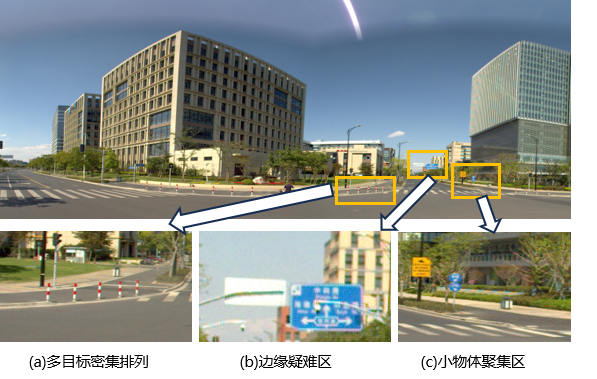
\includegraphics[width=1.0\textwidth]{logo/第二阶段候选裁剪区域推荐示意图.png}
    \caption{第二阶段候选裁剪区域推荐示意图}
    \label{fig:crop_recommendation}
\end{figure}
% =========================================================

\subsection{Crop Agent 的训练目标}
\label{subsec:crop_agent_training_objective}

为了使 Crop Agent 学会生成兼具覆盖性、紧凑性与非冗余性的候选区域，本文先设计裁剪区域价值奖励机制，再将其实现为 \texttt{CropRegionRewardFunction}。该奖励函数由召回项、紧致项、精度项、重叠惩罚项与格式项共同构成：
\begin{equation}
R_{\text{crop}}
=
R_{\text{recall}}
+
R_{\text{compact}}
+
R_{\text{precision}}
+
R_{\text{overlap}}
+
R_{\text{format}}.
\label{eq:crop_reward_total}
\end{equation}

首先，考虑到第二阶段关注的核心是\textbf{小目标是否被裁剪区域覆盖}，本文采用 IoG（Intersection over Ground-truth）而非 IoU 作为覆盖度量。设小目标真实框为 $g_i$，候选裁剪区域为 $c_j$，则二者的 IoG 定义为：
\begin{equation}
\mathrm{IoG}(g_i,c_j)=\frac{|g_i\cap c_j|}{|g_i|}.
\label{eq:iog}
\end{equation}
IoG 反映了真实目标有多少比例被当前裁剪区域覆盖。当裁剪框明显大于真实小目标时，IoU 往往会偏低，而 IoG 更能准确反映“该目标是否已被有效纳入后续局部检测范围”。

基于此，召回项定义为每个真实小目标在全部裁剪区域中的最大覆盖程度平均值：
\begin{equation}
R_{\text{recall}}
=
w_r \cdot \frac{1}{N_g}\sum_{i=1}^{N_g}\max_j \mathrm{IoG}(g_i,c_j),
\label{eq:crop_recall}
\end{equation}
其中，$N_g$ 表示小目标真实框数量，$w_r$ 表示召回项权重。

然而，若仅优化召回项，Crop Agent 很容易退化为输出一个或少数几个极大的裁剪框，从而虽然覆盖了大量目标，但失去了局部精检所需的区域紧致性。为避免这种“大框一把罩”的坍缩解，本文进一步引入紧致项。设某一裁剪区域 $c_j$ 所覆盖的小目标集合为 $\mathcal{G}_j$，由这些目标的最小包围矩形面积记为 $A_{\text{tight},j}$，裁剪区域本身面积记为 $A_{c_j}$，则其紧致度定义为：
\begin{equation}
C_j = \frac{A_{\text{tight},j}}{A_{c_j}}.
\label{eq:compactness}
\end{equation}
由此可得紧致项：
\begin{equation}
R_{\text{compact}}
=
w_c \cdot \frac{1}{|\mathcal{C}^{+}|}\sum_{c_j \in \mathcal{C}^{+}} C_j,
\label{eq:crop_compactness}
\end{equation}
其中，$\mathcal{C}^{+}$ 表示确实覆盖了至少一个真实目标的有效裁剪区域集合，$w_c$ 表示紧致项权重。该项鼓励 Crop Agent 输出能够紧密包围目标群的局部区域，而不是过度扩张的无效大框。

为了进一步减少无效裁剪，本文引入精度项。若某一裁剪区域几乎未覆盖任何真实目标，则应受到惩罚。定义每个裁剪区域的最大匹配 IoG 为：
\begin{equation}
q_j = \max_i \mathrm{IoG}(g_i,c_j),
\label{eq:max_iog_pred}
\end{equation}
则精度惩罚项定义为：
\begin{equation}
R_{\text{precision}}
=
-
w_p \cdot \frac{1}{N_c}\sum_{j=1}^{N_c}(1-q_j),
\label{eq:crop_precision_penalty}
\end{equation}
其中，$N_c$ 表示裁剪区域数量，$w_p$ 为精度项权重。

同时，为防止多个裁剪区域大量重叠、重复关注相同区域，本文还引入重叠惩罚项。设所有裁剪区域之间两两 IoU 的平均值为 $\overline{\mathrm{IoU}}_{\text{crop}}$，则：
\begin{equation}
R_{\text{overlap}} = - w_o \cdot \overline{\mathrm{IoU}}_{\text{crop}},
\label{eq:crop_overlap_penalty}
\end{equation}
其中，$w_o$ 表示重叠惩罚权重。

综上，裁剪奖励函数在训练中同时鼓励 Crop Agent 提高对小目标的覆盖能力、保持候选区域紧凑、减少无效裁剪并抑制冗余重叠，从而使第二阶段输出的候选区域真正具备高补检价值。

% ========================= 图 4-4 =========================
\begin{figure}[htbp]
    \centering
    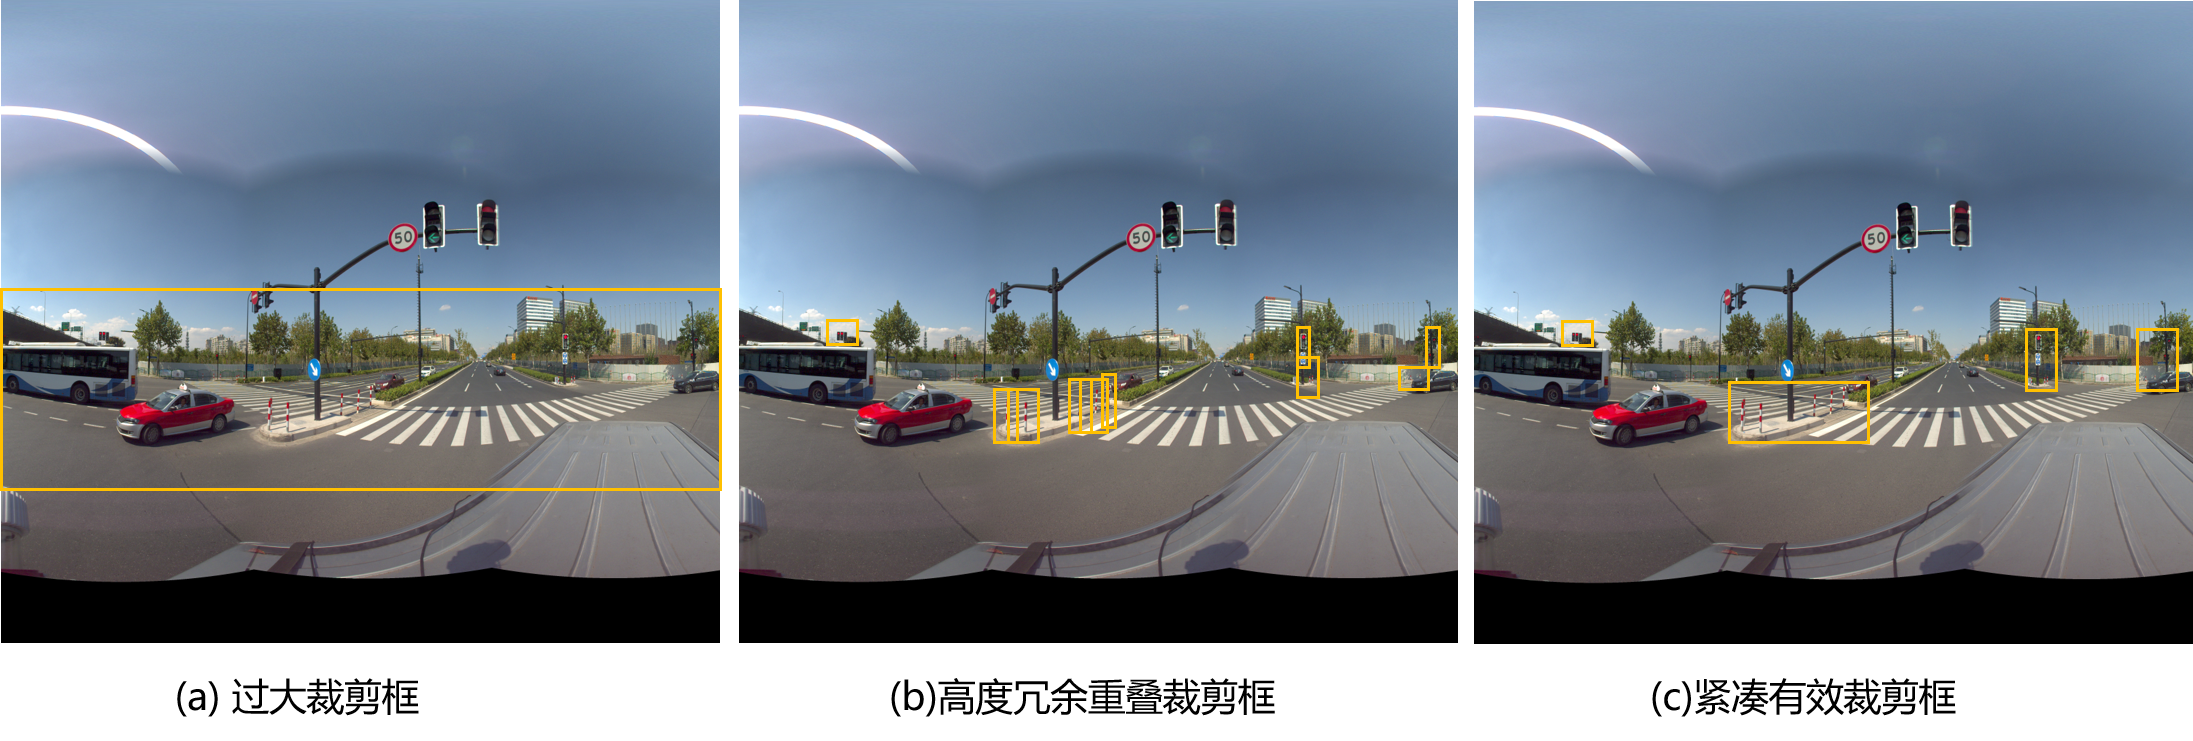
\includegraphics[width=1.0\textwidth]{logo/不同候选裁剪策略的对比示意图.png}
    \caption{不同候选裁剪策略的对比示意图}
    \label{fig:crop_strategy_comparison}
\end{figure}
% =========================================================


\section{第三阶段：基于局部区域的精细检测}
\label{sec:stage3_local_refinement}

\subsection{局部精检机制}
\label{subsec:local_refinement_mechanism}

在第二阶段获得候选裁剪区域后，系统对每个局部区域执行第三阶段检测。与第一阶段面向整图的全局初检不同，第三阶段的输入为局部裁剪后的图像块，此时目标在图像中的有效占比通常得到提高，局部背景干扰则相对减少。因此，第三阶段的检测更适合恢复全图尺度下容易被忽略的小目标、密集目标和边缘目标。

从感知角度看，局部裁剪后的输入具有以下优势。首先，目标的有效成像尺度被放大，目标边界与局部结构更容易被检测器捕获；其次，与全图检测相比，局部输入中的无关背景比例下降，从而减弱了背景噪声对目标分类与定位的干扰；最后，在密集目标区域中，局部精检能够降低多个目标在大尺度特征图上的竞争关系，提高目标之间的可分性。

因此，第三阶段的作用并不是重复第一阶段，而是在 Crop Agent 主动筛选出的高价值区域内执行有针对性的补充检测。其本质是将局部精细观察能力显式引入检测流程，以弥补全局检测在疑难区域中的不足。

\subsection{第三阶段与第一阶段的关系}
\label{subsec:relationship_between_stage1_and_stage3}

尽管第一阶段和第三阶段都由 Detection Agent 完成边界框检测，但二者承担的角色并不相同。第一阶段面向整图，目标是建立场景级初始检测基线；第三阶段面向局部区域，目标是恢复第一阶段可能遗漏的目标。因此，第三阶段在功能上并不是对第一阶段的简单重复，而是一种明确面向漏检恢复的补检机制。

这种关系可进一步理解为：第一阶段提供全局感知与初始结果，第二阶段通过 Crop Agent 将感知资源重新分配给高价值区域，第三阶段再对这些区域执行精细检测。由此，本文方法形成了“\textbf{全局覆盖—局部补充}”的分层检测机制，使检测系统既保持对整体场景的把握能力，又具备对疑难区域进行再次观察的能力。

% ========================= 图 4-5 =========================
\begin{figure}[ht]
  \centering
  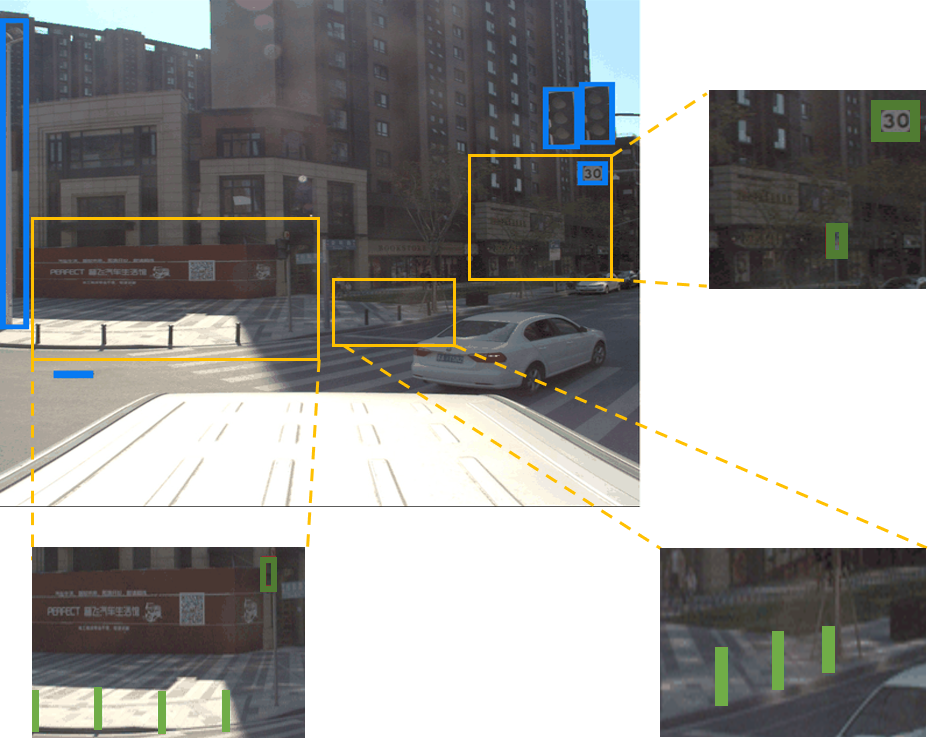
\includegraphics[width=\linewidth]{logo/第三阶段局部精检对遗漏目标的恢复示意图.png}
  \caption{第三阶段局部精检对遗漏目标的恢复示意图}
  \label{fig:my_label_1}
\end{figure}
% =========================================================


\section{三阶段检测结果融合策略}
\label{sec:fusion_strategy}

\subsection{融合规则定义}
\label{subsec:fusion_rule}

由于第一阶段与第三阶段均输出边界框集合，因此需要设计一套后处理机制对二者进行融合。本文采用一种面向增量补检的轻量融合策略：对于第三阶段输出的每一个候选框，若其与第一阶段任一检测框的 IoU 超过阈值 $\tau_f$，则将该框视为重复检测结果并删除；否则，将其作为新增补检框保留。本文中采用的融合阈值为：
\begin{equation}
\tau_f = 0.1.
\label{eq:fusion_threshold}
\end{equation}

因此，经过过滤后的第三阶段检测结果集合可表示为：
\begin{equation}
\mathcal{B}^{(3)\prime}
=
\left\{
b \in \mathcal{B}^{(3)}
\;\middle|\;
\max_{b' \in \mathcal{B}^{(1)}} \mathrm{IoU}(b,b') \le \tau_f
\right\}.
\label{eq:filtered_stage3}
\end{equation}

最终融合结果为：
\begin{equation}
\mathcal{B}^{*} = \mathcal{B}^{(1)} \cup \mathcal{B}^{(3)\prime}.
\label{eq:final_fusion}
\end{equation}

\subsection{融合策略的作用}
\label{subsec:role_of_fusion_strategy}

上述融合规则的核心思想在于：\textbf{第三阶段主要负责补充第一阶段的遗漏结果，而不是重复覆盖第一阶段已检测到的目标}。通过对第三阶段结果进行低阈值去重，可以有效抑制局部检测因尺度变化而带来的重复框问题，同时尽可能保留真正的新增补检结果。

与传统意义上的 NMS 不同，本文的融合步骤并非试图在所有框之间重新竞争最优框，而是更强调第一阶段与第三阶段的功能边界。由于第一阶段已经提供了场景级初始结果，因此第三阶段结果只有在不与第一阶段结果明显重合时，才被视为具有实际增益的补检信息。由此，最终输出结果可以更自然地解释为“全局初检结果 + 局部补检结果”的增量融合。

% ========================= 图 4-6 =========================
\begin{figure}[ht]
  \centering
  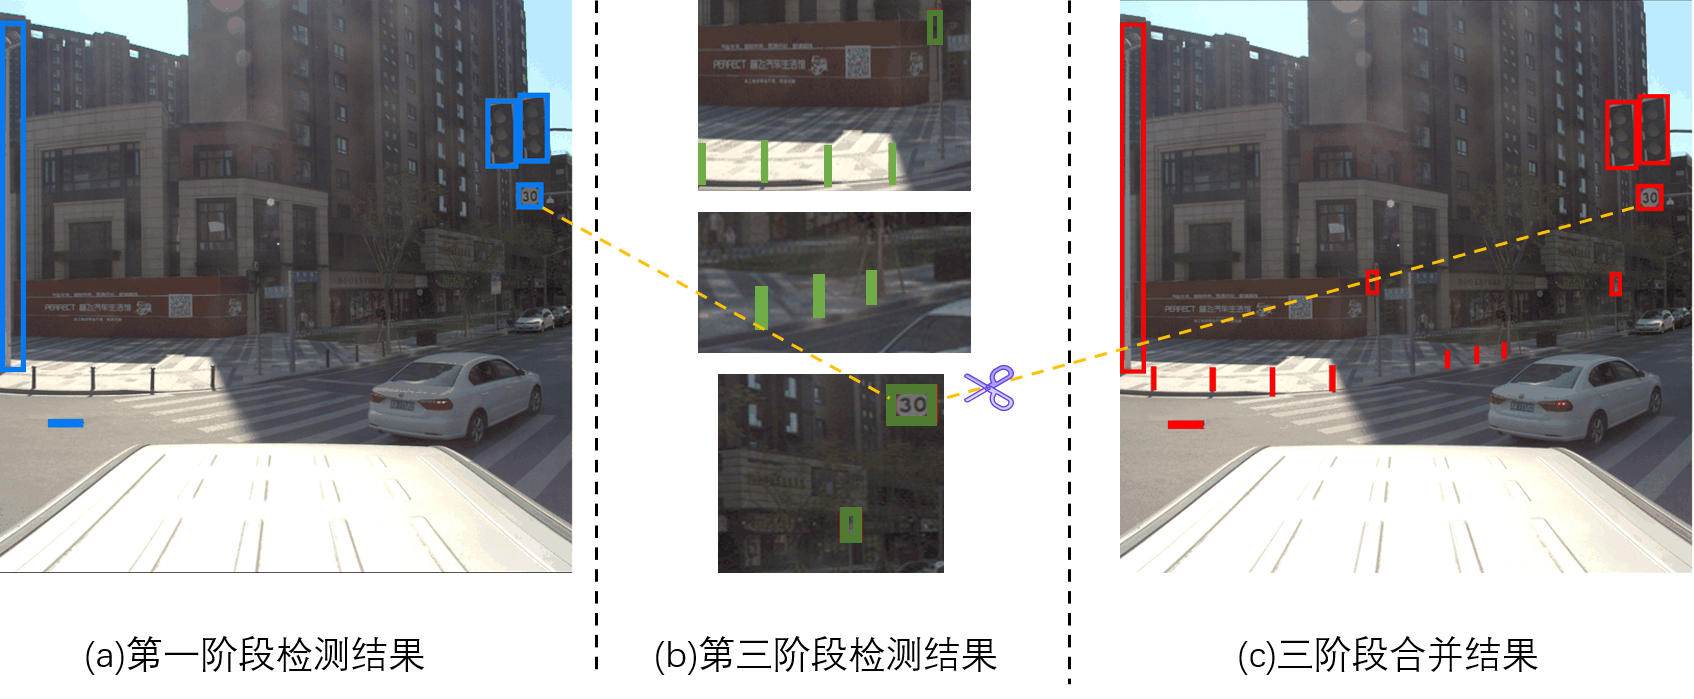
\includegraphics[width=\linewidth]{logo/第一阶段与第三阶段检测结果的融合示意图.png}
  \caption{第一阶段与第三阶段检测结果的融合示意图}
  \label{fig:my_label_2}
\end{figure}
% =========================================================


\section{本章小结}
\label{sec:chapter4_summary}

本章围绕交通资产检测中的小目标易漏检、密集目标难分离以及疑难区域难以充分感知等问题，提出了一种基于主动感知的多智能体交通资产检测框架。该框架由 Detection Agent 与 Crop Agent 两类功能异质的智能体协同构成，将传统的单次全图检测过程扩展为“全局初检—候选区域推荐—局部精检—结果融合”的三阶段主动感知流程。

其中，第一阶段通过全图检测建立场景级初始检测基线；第二阶段由 Crop Agent 根据原图与初检结果主动生成具有高补检价值的候选区域；第三阶段再由 Detection Agent 在局部区域内执行精细检测，从而恢复第一阶段可能遗漏的目标。在模型训练方面，本文分别为 Detection Agent 与 Crop Agent 设计了针对性的奖励函数，以提升检测能力与候选区域推荐能力；在结果输出方面，本文进一步采用面向增量补检的融合策略，对第一阶段与第三阶段检测结果进行统一整合。

总体而言，本章所提出的检测框架并不依赖于某一特定检测模型，而是通过多智能体协作与主动感知机制，为不同类型检测器提供统一的漏检补偿路径，为下一章的实验验证与性能分析奠定了方法基础。

\chapter{交通资产检测实验结果与分析}
\label{chap:experiments}

\section{实验设置}
\label{sec:exp_setup}

\subsection{实验目标}
\label{subsec:exp_goal}

本章围绕第三章提出的“全局初检—候选区域推荐—局部精检—结果融合”三阶段框架展开实验验证，重点回答以下四个问题：

第一，所提出的三阶段主动感知检测框架，是否能够在交通资产检测任务上相较于原始检测器取得稳定性能增益；

第二，该框架对于小目标、密集目标以及复杂背景区域中的目标检测，是否具有更明显的改进效果；

第三，该框架是否具有检测器无关性，即能否在不同类型的 Detection Agent 上均表现出一致有效性；

第四，框架中各关键组成部分，尤其是候选区域推荐与局部精检机制，分别对最终性能起到了怎样的作用。

为回答上述问题，本文从整体性能对比、小目标与密集目标分析、异构检测器泛化分析、消融实验以及可视化结果分析五个层面展开实验。

\subsection{数据集与评价设置}
\label{subsec:dataset_metric_setting}

本文实验均在交通资产检测数据集上进行评估。训练阶段使用武汉数据集，测试阶段使用上海数据集，以验证模型在跨城市域偏移条件下的泛化能力。数据集中包含路灯、交通标志、交通灯、井盖、消火栓、监控设备、锥桶、垃圾桶、路桩等多类道路基础设施目标，具有小目标占比高、尺度变化大、目标分布密集以及局部背景复杂等特点。

为了更细致地反映模型在不同尺度目标上的检测能力，本文采用分尺度评估策略。具体而言，当目标长宽均大于给定阈值时，将其视为大目标；否则视为小目标。评价时采用差异化 IoU 匹配阈值：大目标使用 IoU=0.5，小目标使用 IoU=0.1。该设置与本文任务中小目标占比较高、且边界框轻微偏移即可导致常规 IoU 严重下降的特点相一致。

在评价指标方面，本文主要采用 Precision、Recall、F1-score、mIoU 以及 Micro-IoU。其定义如下：
\begin{equation}
\mathrm{Precision}=\frac{TP}{TP+FP},
\qquad
\mathrm{Recall}=\frac{TP}{TP+FN},
\label{eq:precision_recall_exp}
\end{equation}

\begin{equation}
F1=\frac{2\cdot \mathrm{Precision}\cdot \mathrm{Recall}}
{\mathrm{Precision}+\mathrm{Recall}},
\label{eq:f1_exp}
\end{equation}

\begin{equation}
\mathrm{IoU}_c=\frac{TP_c}{TP_c+FP_c+FN_c},
\label{eq:iou_exp}
\end{equation}

\begin{equation}
mIoU=\frac{1}{C}\sum_{c=1}^{C}\mathrm{IoU}_c,
\label{eq:miou_exp}
\end{equation}
其中，$TP$、$FP$ 和 $FN$ 分别表示真阳性、假阳性和假阴性数量，$C$ 表示类别数。

为明确区分 Macro 与 Micro 统计口径，本文进一步定义：
\begin{equation}
F1_c=\frac{2P_cR_c}{P_c+R_c},\qquad
\mathrm{Macro\text{-}F1}=\frac{1}{C}\sum_{c=1}^{C}F1_c,
\label{eq:macro_f1_exp}
\end{equation}
\begin{equation}
\mathrm{Micro\text{-}F1}
=\frac{2\sum_{c=1}^{C}TP_c}
{2\sum_{c=1}^{C}TP_c+\sum_{c=1}^{C}FP_c+\sum_{c=1}^{C}FN_c},
\label{eq:micro_f1_exp}
\end{equation}
\begin{equation}
\mathrm{Micro\text{-}IoU}
=\frac{\sum_{c=1}^{C}TP_c}
{\sum_{c=1}^{C}TP_c+\sum_{c=1}^{C}FP_c+\sum_{c=1}^{C}FN_c}.
\label{eq:micro_iou_exp}
\end{equation}

其中，Macro-F1 对每个类别赋予相同权重，更能反映长尾类别与小样本类别的整体表现；Micro-F1 对所有样本统一汇总，更偏向反映高频类别上的总体识别效果。类似地，mIoU 是“先按类别计算 IoU 再平均”，强调各类别均衡性；Micro-IoU 是“全类别 TP/FP/FN 汇总后计算 IoU”，更强调全局检测质量与主流类别贡献。

\subsection{对比方法}
\label{subsec:compared_methods}

为了验证所提出框架的泛化能力，本文选取了六种类型差异较大的检测器作为 Detection Agent：rexomini\cite{rexomni2025}、DINO\cite{zhang2022dino}、Faster R-CNN\cite{ren2015faster}、DEIM\cite{huang2025deim}、Grounding DINO\cite{liu2024grounding} 和 YOLO26\cite{ultralytics2026yolo26}。对所有模型，均分别评估其原始检测结果，以及接入本文“全局初检—候选区域推荐—局部精检—结果融合”三阶段流程后的增强结果。实验执行顺序严格遵循两阶段协议：先完成“rexomini Detection Agent + rexomini Crop Agent”的同源训练与验证，再扩展到“固定 Crop Agent、替换 Detection Agent”的异构检测器对比。

需要强调的是，本文方法不改动基础检测器的检测头结构。实验核心不是比较不同 backbone/neck，而是比较“\textbf{原始检测器}”与“\textbf{原始检测器 + 三阶段主动感知框架}”的差异。

此外，本文的 Crop Agent 并非从零训练，而是由已训练好的 rexomini 检测 Agent 继续训练得到。其原因是：预训练检测 Agent 已具备“物体大致位置感知”能力，继续训练时只需将优化目标切换为三类高价值区域推荐——边缘疑难区、小物体聚集区和多目标密集区。为保证可比性，本章实验中 Crop Agent 保持固定，仅替换第一、三阶段的 Detection Agent。需要特别强调的是，被替换的 DINO、Faster R-CNN、DEIM、Grounding DINO 和 YOLO26 均采用各自模型原始训练方式（即各自论文/官方常规训练范式），不额外进行本文的 \texttt{BoxIoURewardFunction} 或 \texttt{CropRegionRewardFunction} 强化学习训练。

\begin{table}[htbp]
    \centering
    \caption{实验中采用的对比检测器}
    \label{tab:compared_detectors}
    \begin{tabular}{llll}
        \toprule
        检测器 & 类型 & 在框架中的角色 & 实验配置 \\
        \midrule
        rexomini & 大模型检测器 & Detection Agent & 原始 / 接入三阶段框架 \\
        DINO & Transformer 检测器 & Detection Agent & 原始 / 接入三阶段框架 \\
        Faster R-CNN & 两阶段检测器 & Detection Agent & 原始 / 接入三阶段框架 \\
        DEIM & 通用目标检测器 & Detection Agent & 原始 / 接入三阶段框架 \\
        Grounding DINO & 开放词汇检测器 & Detection Agent & 原始 / 接入三阶段框架 \\
        YOLO26 & 单阶段检测器 & Detection Agent & 原始 / 接入三阶段框架 \\
        \bottomrule
    \end{tabular}
\end{table}

\subsection{实现细节}
\label{subsec:implementation_details}

在实验过程中，本文统一遵循第三章提出的三阶段检测流程。第一阶段在整幅图像上执行全局初检，得到初始检测框集合；第二阶段由 Crop Agent 根据原图与初检结果生成候选裁剪区域；第三阶段在候选区域内执行局部精检；最终通过结果融合策略获得最终检测输出。

为保证不同检测器之间的实验具有可比性，本文在所有对比模型上尽可能保持一致的候选区域生成逻辑、裁剪数量控制规则以及融合策略。特别地，在结果融合阶段，首先将第三阶段局部检测结果映射回原图坐标系，再与第一阶段检测结果进行重复框筛除；当第三阶段检测框与第一阶段任一检测框的 IoU 小于固定阈值 $\tau_f=0.1$ 时，该框才作为新增补检结果保留，否则视为重复检测并删除，从而避免重复框对最终统计结果造成干扰。


\section{整体性能对比}
\label{sec:overall_comparison}

\subsection{总体结果分析}
\label{subsec:overall_result_analysis}

表~\ref{tab:overall_main_results} 给出了不同检测器在原始检测设置与接入本文框架后的整体性能对比结果。总体来看，三阶段主动感知流程在多种类型 Detection Agent 上均能够带来稳定性能提升，说明该方法并非仅对特定检测器有效，而具有较好的检测器无关性与泛化能力。

从六个检测器的结果看，Macro-F1、Micro-F1、mIoU 和 Micro-IoU 均呈现提升趋势，平均绝对增益分别为 +8.18\%、+6.41\%、+2.90\% 和 +2.53\%。这一结果具有两层含义：其一，Macro-F1 增益高于 Micro-F1，说明改进并非只来自高频类别，而是对长尾类别也有实质补益；其二，mIoU 与 Micro-IoU 同步上升，表明提升不仅体现在“检出来更多”，也体现在“框匹配更合理”。

从结果性质上看，这种提升并不意味着框架仅通过增加预测框数量获得收益，而是说明通过“候选区域推荐 + 局部精检”机制，模型能够在原始全图检测基础上有效恢复部分遗漏目标，尤其是在小尺度和复杂区域目标上提升 Recall，并在合理控制 Precision 波动的前提下推动整体 F1 提升。

进一步观察不同模型的收益幅度可以发现：Faster R-CNN、DEIM、DINO 和 YOLO26 的增幅更大；Grounding DINO 与 rexomini 在较高基线下仍保持稳定提升。以 Grounding DINO 为例，其 Micro-F1 从 0.7665 提升至 0.7816，mIoU 从 0.4944 提升至 0.5154，说明即使在强基线模型上，局部再检测与增量融合机制仍然有效。

结合“武汉训练—上海测试”的跨城设置，这些结果进一步说明：本文方法并非依赖单一模型结构，而是在明显域偏移下仍能稳定提升检测完整性与匹配质量，具有较好的跨场景泛化潜力。

\begin{table}[htbp]
    \centering
    \caption{不同检测器接入本文框架前后的整体性能对比}
    \label{tab:overall_main_results}
    \resizebox{\textwidth}{!}{
    \begin{tabular}{lcccccccccccc}
        \toprule
        \multirow{2}{*}{检测器} & \multicolumn{3}{c}{Macro-F1} & \multicolumn{3}{c}{Micro-F1} & \multicolumn{3}{c}{mIoU} & \multicolumn{3}{c}{Micro-IoU} \\
        \cmidrule(lr){2-4} \cmidrule(lr){5-7} \cmidrule(lr){8-10} \cmidrule(lr){11-13}
        & 前 & 后 & $\Delta$(\%) & 前 & 后 & $\Delta$(\%) & 前 & 后 & $\Delta$(\%) & 前 & 后 & $\Delta$(\%) \\
        \midrule
        rexomini & 0.6148 & 0.6328 & +1.80 & 0.6770 & 0.6853 & +0.83 & 0.3705 & 0.3828 & +1.23 & 0.4231 & 0.4264 & +0.33 \\
        DINO & 0.5308 & 0.5778 & +4.70 & 0.5878 & 0.6354 & +4.76 & 0.3163 & 0.3531 & +3.68 & 0.3668 & 0.4057 & +3.89 \\
        Faster R-CNN & 0.1322 & 0.3803 & +24.81 & 0.2515 & 0.4370 & +18.55 & N/A & N/A & N/A & N/A & N/A & N/A \\
        DEIM & 0.4265 & 0.5300 & +10.35 & 0.5108 & 0.5940 & +8.32 & 0.2322 & 0.3000 & +6.78 & 0.2934 & 0.3524 & +5.90 \\
        Grounding DINO & 0.7279 & 0.7486 & +2.07 & 0.7665 & 0.7816 & +1.51 & 0.4944 & 0.5154 & +2.10 & 0.5360 & 0.5525 & +1.65 \\
        YOLO26 & 0.4345 & 0.4879 & +5.34 & 0.5206 & 0.5654 & +4.48 & 0.2504 & 0.2863 & +3.59 & 0.3153 & 0.3493 & +3.40 \\
        \bottomrule
    \end{tabular}}
\end{table}

\subsection{大目标与整体结果的关系}
\label{subsec:large_vs_overall}

进一步观察分尺度统计结果可以发现，本文方法的主要收益并非来自大目标重复检测，而是来自小目标与疑难区域补检。六个检测器中，大目标 Micro-F1 平均增益仅为 +0.04\%，而小目标 Micro-F1 平均增益为 +9.30\%，显著更高。

这一现象与本文方法设计初衷一致：第一阶段建立全局检测基线，第二、三阶段将计算资源聚焦到“边缘疑难区、小物体聚集区、多目标密集区”。因此，本文框架可以被视为一种面向漏检恢复的增量式增强策略。

\begin{table}[htbp]
    \centering
    \caption{不同检测器在分尺度下的增益对比（单位：\%）}
    \label{tab:yolo_scale_results}
    \begin{tabular}{lcccc}
        \toprule
        检测器 & $\Delta$大目标 Micro-F1 & $\Delta$小目标 Micro-F1 & $\Delta$整体 Micro-F1 & $\Delta$小目标 Recall \\
        \midrule
        rexomini & -0.07 & +1.30 & +0.83 & +5.56 \\
        DINO & +0.07 & +6.66 & +4.76 & +9.05 \\
        Faster R-CNN & +0.31 & +27.39 & +18.55 & +25.17 \\
        DEIM & -0.04 & +11.97 & +8.32 & +14.80 \\
        Grounding DINO & -0.09 & +2.12 & +1.51 & +5.32 \\
        YOLO26 & +0.08 & +6.33 & +4.48 & +6.73 \\
        \bottomrule
    \end{tabular}
\end{table}


\section{小目标与密集目标检测性能分析}
\label{sec:small_dense_analysis}

\subsection{小目标检测性能提升分析}
\label{subsec:small_object_analysis}

交通资产检测场景中，大量目标具有尺寸小、纹理弱、与背景相似度高等特点，这使得小目标检测成为评价检测系统实用性的关键环节。本文提出的三阶段主动感知框架，正是针对这类目标在全图检测中容易被忽略的问题而设计。

从六个检测器的小目标结果看，提升主要体现为 Recall 增长并带动 F1 提升。以 DEIM 为例，小目标 Recall 从 0.3389 提升至 0.4869（+14.80\%），Micro-F1 从 0.4442 提升至 0.5639（+11.97\%）；YOLO26 的小目标 Recall 从 0.3344 提升至 0.4017（+6.73\%），Micro-F1 从 0.4528 提升至 0.5161（+6.33\%）；DINO 的小目标 Recall 从 0.4346 提升至 0.5251（+9.05\%），Micro-F1 从 0.5302 提升至 0.5968（+6.66\%）。该现象说明主动裁剪与局部精检能够有效恢复全图检测遗漏的小尺度目标。

值得注意的是，小目标提升并不是通过简单放宽阈值或堆叠预测框获得，而是通过候选区域推荐机制将检测资源重新分配到高价值局部区域。在局部裁剪后，小目标有效尺度被放大、背景干扰被压缩，因此不同检测器都能获得一致的小目标补检收益。

\begin{table}[htbp]
    \centering
    \caption{不同检测器在小目标上的性能对比}
    \label{tab:yolo_small_results}
    \resizebox{\textwidth}{!}{
    \begin{tabular}{lcccccc}
        \toprule
        检测器 & Recall（前） & Recall（后） & $\Delta$Recall（\%） & Micro-F1（前） & Micro-F1（后） & $\Delta$Micro-F1（\%） \\
        \midrule
        rexomini & 0.5667 & 0.6223 & +5.56 & 0.6489 & 0.6619 & +1.30 \\
        DINO & 0.4346 & 0.5251 & +9.05 & 0.5302 & 0.5968 & +6.66 \\
        Faster R-CNN & 0.0860 & 0.3377 & +25.17 & 0.1368 & 0.4107 & +27.39 \\
        DEIM & 0.3389 & 0.4869 & +14.80 & 0.4442 & 0.5639 & +11.97 \\
        Grounding DINO & 0.6408 & 0.6940 & +5.32 & 0.7403 & 0.7615 & +2.12 \\
        YOLO26 & 0.3344 & 0.4017 & +6.73 & 0.4528 & 0.5161 & +6.33 \\
        \bottomrule
    \end{tabular}}
\end{table}

从表~\ref{tab:yolo_small_results} 可见，六个检测器的小目标 Recall 全部为正增益，进一步验证了本文方法的核心作用是“漏检恢复”。虽然部分模型的 Precision 会有轻微波动，但 Recall 的提升幅度更大，因此最终 F1 普遍上升。

\subsection{密集目标与复杂区域分析}
\label{subsec:dense_region_analysis}

除小目标外，密集目标区域同样是交通资产检测中的典型难点。此类区域往往包含多个相邻目标、结构相似目标或者排列紧凑目标，模型在全图尺度下容易出现相互遮蔽、重复抑制或部分遗漏等问题。

本文框架对这类区域的改进主要体现在两个方面。首先，Crop Agent 候选区域推荐机制能够主动识别高密度目标分布区域，并将这些区域作为第三阶段重点检测对象；其次，局部精检阶段能够在更小视野内重新解析目标间的边界关系，从而提升相邻目标之间的可分性。对于交通标志群、连续路灯、密集路桩以及复杂路侧设施区域，这种机制通常能够带来更好的目标分离效果。

从实验现象看，接入本文三阶段检测框架后的结果在复杂道路边缘区域、远距离设施聚集区域以及多目标并列区域中，能够恢复更多此前被遗漏的目标。这说明主动感知机制不仅提高了单个小目标的被发现概率，也改善了复杂区域的整体可解析性。

% ======================== 图建议 5-2 ========================
\begin{figure}[htbp]
    \centering
    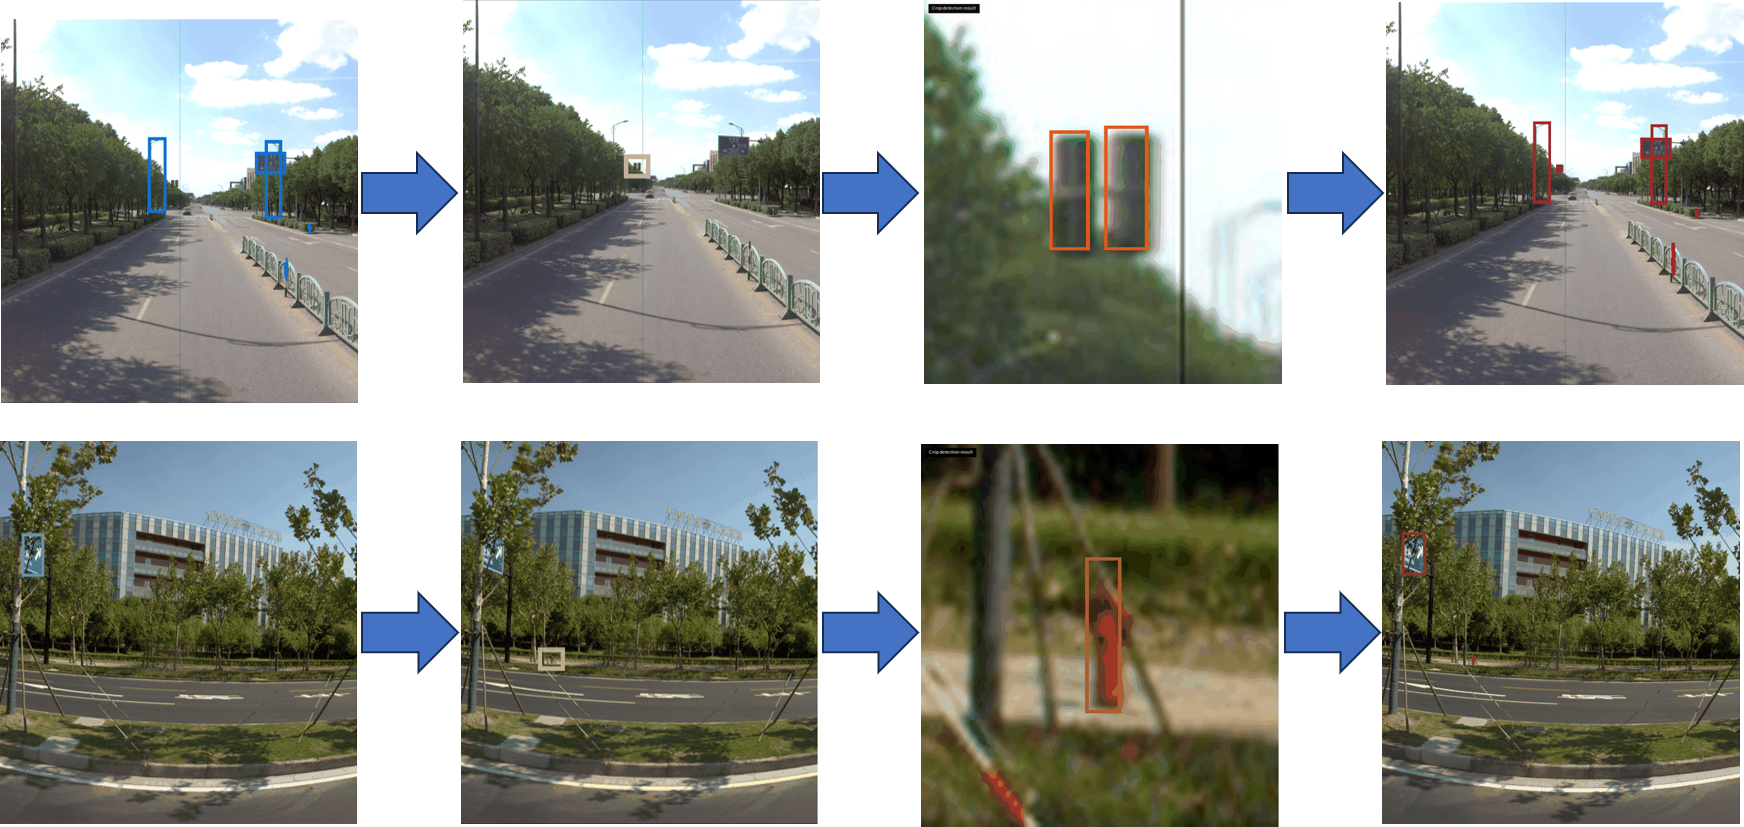
\includegraphics[width=1.0\textwidth]{logo/小目标检测结果可视化对比.png}
    
    \caption{小目标检测结果可视化对比}
    \label{fig:small_object_cases}
\end{figure}
% ==========================================================

% ======================== 图建议 5-3 ========================
\begin{figure}[htbp]
    \centering
    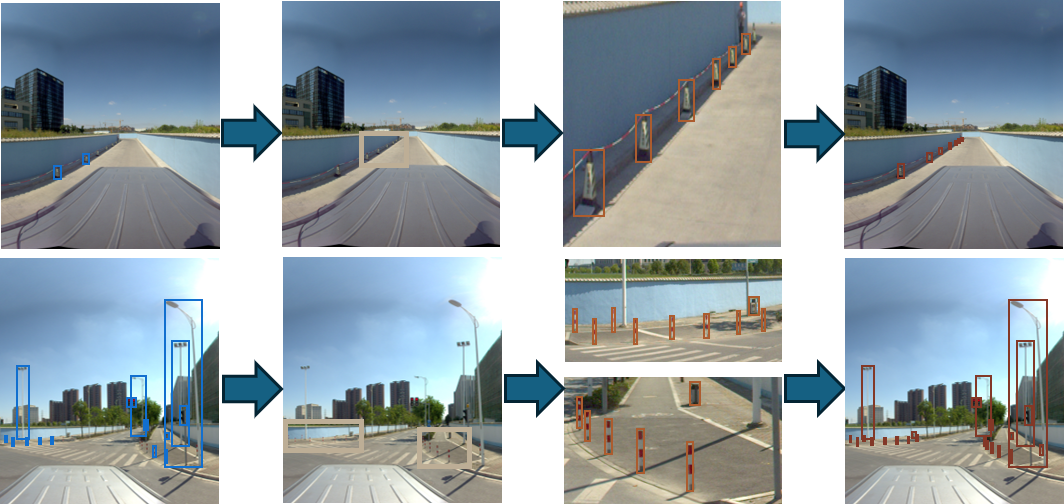
\includegraphics[width=1.0\textwidth]{logo/密集区域检测结果可视化对比.png}
    \caption{密集区域检测结果可视化对比}
    \label{fig:dense_region_cases}
\end{figure}
% ==========================================================


\section{异构 Detection Agent 上的泛化能力分析}
\label{sec:generalization_analysis}

\subsection{跨检测器一致增益分析}
\label{subsec:cross_detector_gain}

本文方法的一个重要特点在于其并不依赖于某一特定检测器的内部结构，而是通过在检测器外部引入主动感知式补检流程，实现对不同 Detection Agent 的统一增强。从实验对比结果可以看出，无论基础模型属于大模型检测器、单阶段检测器、两阶段检测器还是开放词汇检测器，接入本文框架后均能够获得不同程度的性能提升。

这一结果说明，本文框架所解决的并不是某一类检测器特有的偏差问题，而是交通资产检测场景中的一个更普遍问题：\textbf{单次全图检测往往难以兼顾全局覆盖与局部精检}。不同模型虽然在特征提取方式、候选生成方式和回归头结构上有所不同，但它们在面对小目标、密集目标和复杂局部区域时，都会不同程度地存在感知不足的问题。本文提出的三阶段主动感知框架，本质上是在检测器之外提供了一种统一的二次观察机制，因此能够在多类检测器上表现出一致有效性。

\subsection{对大模型检测器与通用检测器的适配性}
\label{subsec:vlm_and_classic_detector_adaptability}

进一步从模型类型角度看，本文方法对大模型检测器与传统视觉检测器都具有良好适配性。对于 rexomini 与 Grounding DINO 这类强基线模型，框架在较高起点上继续带来稳定增益；对于 DINO、DEIM、YOLO26 和 Faster R-CNN，增益幅度更大，说明该机制对“基线漏检较多”的检测器尤为有效。

同时，本章实验还体现了一个关键工程事实：Crop Agent 作为第二阶段核心模块，采用“基于已训练 Detection Agent 继续训练”的路径更稳定。本文使用由 rexomini 继续训练得到的 Crop Agent，在不更换 Crop Agent 的条件下，对六种 Detection Agent 均取得增益，说明该 Crop 策略具有较强可迁移性。换言之，本章结论中的“可迁移性”是指在固定 rexomini 训练得到的 Crop Agent 前提下，对异构 Detection Agent 的外部增强有效，而非意味着所有检测器均经过了同构强化学习训练。

需要说明的是，本文关于 Crop Agent 可迁移性的结论，主要限定于“固定由 rexomini 继续训练得到的 Crop Agent，对异构 Detection Agent 产生外部增强效果”这一实验事实，而不进一步推广到所有类型裁剪策略。

这表明，本文提出的主动感知框架具有较强的模型兼容性与部署灵活性。在实际应用中，系统可以根据检测任务需求选择适合的 Detection Agent，而无需重新设计主动感知逻辑本身。

\begin{table}[htbp]
    \centering
    \caption{异构 Detection Agent 上的性能增益统计（单位：\%）}
    \label{tab:heterogeneous_gain}
    \begin{tabular}{lcccc}
        \toprule
        检测器 & $\Delta$Macro-F1 & $\Delta$Micro-F1 & $\Delta$mIoU & $\Delta$Micro-IoU \\
        \midrule
        rexomini & +1.80 & +0.83 & +1.23 & +0.33 \\
        DINO & +4.70 & +4.76 & +3.68 & +3.89 \\
        Faster R-CNN & +24.81 & +18.55 & N/A & N/A \\
        DEIM & +10.35 & +8.32 & +6.78 & +5.90 \\
        Grounding DINO & +2.07 & +1.51 & +2.10 & +1.65 \\
        YOLO26 & +5.34 & +4.48 & +3.59 & +3.40 \\
        \bottomrule
    \end{tabular}
\end{table}


\section{消融实验}
\label{sec:ablation_study}

\subsection{三阶段结构有效性分析}
\label{subsec:ablation_three_stage}

为验证本文所提出三阶段主动感知检测流程的结构有效性，本节将“全图检测两次并融合”与“完整三阶段框架”进行对比。其中，前者表示在相同 Detection Agent 下，两次检测都直接作用于原始整图，并将两次全图检测结果进行统一融合；后者则采用第一阶段全图初检、第二阶段候选区域推荐、第三阶段局部精检以及最终结果融合的完整流程。

该对比的核心目的在于区分“检测次数增加”与“主动感知策略引入”这两种因素的作用。若仅将检测器在全图上重复执行一次，系统虽然增加了推理次数，但并未改变观测尺度与注意力分配方式；而完整三阶段框架则通过候选区域推荐与局部精检，将第二次观察聚焦到更可能存在遗漏目标的局部区域。

因此，该组实验关注的问题是：在不改变基础 Detection Agent 的前提下，完整三阶段框架的性能提升是否真正来源于“候选区域推荐—局部复查—结果融合”这一主动感知闭环，而非仅仅来自额外增加一次检测。若完整三阶段框架优于“全图检测两次并融合”，则说明本文方法的优势在于局部高价值区域的针对性再检测，而不是简单重复全图推理。

\begin{table}[htbp]
    \centering
    \caption{三阶段主动感知框架结构消融实验}
    \label{tab:ablation_framework}
    \begin{tabular}{lcccc}
        \toprule
        方法设置 & Macro-F1 & Micro-F1 & mIoU & Micro-IoU \\
        \midrule
        全图检测两次并融合 & -- & -- & -- & -- \\
        完整三阶段框架 & -- & -- & -- & -- \\
        \bottomrule
    \end{tabular}
\end{table}

\subsection{裁剪 Agent 有效性对比}
\label{subsec:ablation_crop_agent}

除三阶段整体结构外，本文还进一步比较 Crop Agent 引导裁剪与简单规则裁剪之间的差异。结合实际实验设置，本文设计如下两种对比方案：

\begin{enumerate}
    \item \textbf{均匀四分裁剪检测}：将整幅图像平均划分为四个子块，对四个区域分别执行检测，并将四个区域的检测结果映射回原图后直接合并；
    \item \textbf{Crop Agent 引导的三阶段检测}：先进行第一阶段全图初检，再由第二阶段裁剪模型预测候选区域，最后在第三阶段对候选区域执行局部精检并与初检结果融合。
\end{enumerate}

实验选取 Grounding DINO 与 YOLO26 作为代表性 Detection Agent，分别对应开放词汇检测器与实时单阶段检测器。这样的对比可以更直接回答：若仅通过固定规则提升局部分辨率，能否达到与主动候选区域选择相近的效果；以及 Crop Agent 的性能收益是否来自其对高价值区域的自适应定位能力。

需要说明的是，均匀四分裁剪检测并不属于本文三阶段框架，因为该方法不包含“全图初检—候选区域推荐—局部精检”的闭环，而是直接对四个固定子区域进行检测并合并结果。理论上，这种方法虽然能够在一定程度上提升局部分辨率，但其区域划分方式固定，难以针对小目标密集区、边缘疑难区和非均匀分布目标进行自适应聚焦；相比之下，Crop Agent 引导的三阶段检测能够根据场景内容动态组织高价值候选区域，因此应当取得更优的最终检测结果。

\begin{table}[htbp]
    \centering
    \caption{不同候选裁剪策略下的检测性能对比}
    \label{tab:ablation_crop_agent}
    \begin{tabular}{llcccc}
        \toprule
        检测器 & 方法设置 & Macro-F1 & Micro-F1 & mIoU & Micro-IoU \\
        \midrule
        Grounding DINO & 均匀四分裁剪检测并合并 & -- & -- & -- & -- \\
        Grounding DINO & Crop Agent 引导的三阶段检测 & -- & -- & -- & -- \\
        YOLO26 & 均匀四分裁剪检测并合并 & -- & -- & -- & -- \\
        YOLO26 & Crop Agent 引导的三阶段检测 & -- & -- & -- & -- \\
        \bottomrule
    \end{tabular}
\end{table}

\section{方法有效性与局限性分析}

\subsection{典型成功案例分析}
\label{subsec:success_case_analysis}

本文方法的典型成功案例主要集中在以下三类场景中：

第一类是远距离小目标恢复场景。例如远处交通灯、细长路桩和小型监控设备，在全图检测中常因目标尺寸过小而被忽略，而在局部裁剪后则能够被成功识别。

第二类是密集目标分离场景。例如多个相邻交通标志、连续排列路灯或路侧设施聚集区域，局部精检有助于重新分离相邻目标边界，减少漏检与粘连。

第三类是图像边缘与局部复杂背景场景。在此类区域中，目标往往只占据局部视野的一部分，且背景纹理干扰较强。通过候选区域推荐与局部检测，模型能够获得更聚焦的感知视野，从而提升检测稳定性。

\subsection{局限性分析}
\label{subsec:failure_case_analysis}

尽管本文方法在多数场景中均能够带来性能提升，但仍存在一定局限性。首先，当原始检测器对某些极端困难目标完全缺乏初始感知线索时，第二阶段候选区域推荐可能无法稳定捕获最优局部区域；其次，若局部区域内部背景极为复杂，或者目标本身存在严重遮挡与极端模糊，第三阶段局部精检的提升空间也会受到限制。

此外，在少数情况下，第三阶段局部检测可能引入与第一阶段部分重叠但并非完全重复的候选框，这说明候选区域选择与结果融合策略仍会对最终输出稳定性产生直接影响。


\section{本章小结}
\label{sec:exp_summary}

本章围绕前文提出的基于主动感知的多智能体交通资产检测框架开展了系统实验验证。实验结果表明，本文方法在多种类型的 Detection Agent 上均能够带来稳定性能提升，说明其具有较好的检测器无关性与泛化能力。

在整体性能方面，六个检测器的 Macro-F1、Micro-F1、mIoU 与 Micro-IoU 均呈正增益，证明三阶段机制能够稳定提升检测完整性与匹配质量；在分尺度结果上，小目标收益显著高于大目标，验证了本文框架“面向漏检恢复”的设计定位；在异构检测器实验中，固定 Crop Agent 仍能对不同 Detection Agent 持续增益，说明该策略具有可迁移性；在可视化分析中，本文方法可恢复原始检测器在远距离小目标、密集区域目标及复杂局部区域中的部分遗漏结果。

总体而言，本章实验结果充分证明了本文框架在交通资产检测任务中的有效性，也验证了主动感知三阶段机制在小目标漏检恢复、复杂区域补检以及跨检测器增强方面的实际价值。
